
%\documentclass{acm_proc_article-sp}
\documentclass[11pt,letterpaper]{article}

%==================================
% packages go here
%==================================

\usepackage{url}
\usepackage{graphicx}
\usepackage{cite} % sort citation numbers
\usepackage{color}
\usepackage{soul}
\usepackage{naaclhlt2012}
\usepackage{times}
\usepackage{latexsym}

%\usepackage{ntheorem}
%\usepackage{amsthm}
%\usepackage{multirow} % for complex tables
%\usepackage{times}
%\usepackage[pdftex]{hyperref}
%\hypersetup{colorlinks=false, pdfborder= 0 0 0}
%\usepackage[draft,inline,nomargin]{fixme}
%\newcommand{\hlfixme}[1]{\fixme{\hl{#1}}}
%\newcommand{\hlfxnote}[1]{\fxnote{\hl{#1}}}

%\newcommand{\name}{\emph{Watson Jr.}}
\newcommand{\name}{\emph{DeanQA~}}

\setlength\titlebox{6.5cm}    % Expanding the titlebox

%==================================

%\begin{document}

\title{\name: \\An Advanced Question Answering System}

\author{
	Yann Le Gall\\
    University of Pittsburgh\\	
	Department of Computer Science\\
	6503 Sennot Square\\
    {\tt ylegall@cs.pitt.edu}
\And
	Eric Heim\\
    University of Pittsburgh\\	
    Department of Computer Science\\
	5324 Sennot Square\\
    {\tt eth13@cs.pitt.edu}
	\\
\And
	Alex Conrad\\
    University of Pittsburgh\\
    Department of Computer Science\\
    5422 Sennot Square\\
    {\tt conrada@cs.pitt.edu}
}

\date{12 December 2011}

\begin{document}

\maketitle

%==================================

%\begin{abstract}
%abstract goes here
%\end{abstract}

% A category with the (minimum) three required fields
%\category{I.2}{Artifical Intelligence}{Natural Language Processing}
%\terms{Algorithms, Experimentation}
%\keywords{Question Answering}

%==================================

\section{Introduction}
\label{sec:intro}
\paragraph{}
In this paper, we design, implement, and evaluate a question answering
(QA) system, \name. In our approach, we use several different strategies from
different domains to select potential answers. Then, we employ a
majority voting scheme to combine the results.

% TODO: should this description of the dataset go in another section?
To train and test our QA system, we used the ``CBC Reading
Comprehension Corpus''. This corpus is composed of 125 news stories,
each accompanied by a set of 6-10 factoid questions (e.g. questions
that begin with ``Who'', ``When'', ``Where'', etc.).
%The news stories were obtained from the ``CBC 4 Kids'' website,
%hosted by the Canadian Broadcast Corporation. The questions and an
%answer key were added by the MITRE Corporation, and are in the style
%of actual reading comprehension tests that are given to grade school
%children in the United States.

All stories in the dataset were been split into sentences (one
sentence per line) using the MXTERMINATOR sentence splitter developed
by Adwait Ratnaparkhi.  Paragraphs from the original story are
separated by an empty line. 

The rest of this paper is organized as follows: in
\S\ref{sec:implementation} we describe the design and implementation
of our QA system and each of its sub-components. Next, in
\S\ref{sec:evaluation} we evaluate our system on the test dataset and
present the performance results. Finally, we conclude in
\S\ref{sec:conclusion}.


\section{Implementation}
\label{sec:implementation}
\paragraph{}
In this section we discuss the design and implementation of \name
. First, we explain the general, overall structure. Then we give
a detailed description of the sub-components (\emph{AnswerFinders}) of
the system. Finally, we present our technique for combining the
potential answers from each sub-component.

\begin{figure} 
	\centering
	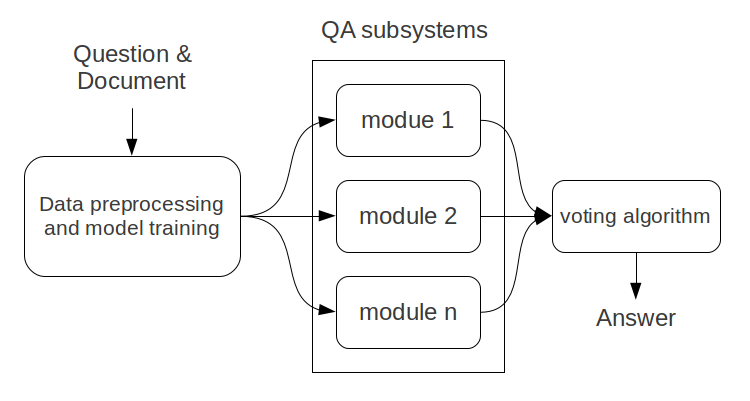
\includegraphics[width=0.45\textwidth]{model.eps}
	\caption{The \name system model.}
	\label{fig:model}
\end{figure}

Figure \ref{fig:model} shows the general design of \name.
The system takes processes a document and a set of questions as input.
At this point, several preprocessing steps might be performed,
including the removal of stop words, coreference resolution, etc.
Next, the processed document and the current question are passed to
each of the AnswerFinders. Each of these AnswerFinders implements a
different strategy for finding answers to the question, and they
each return a collection of \texttt{<answer,confidence>} pairs.
Finally, the potential answers are combineded in a voting algorithm
that gives different weights to the potential answers based on the
confidence and the question type.

In the next few subsections, we give more detailed descriptions of
the implementation of the different AnswerFinders and the
strategies that they use.

\subsection{Bag-of-Words}
\paragraph{}
The Bag-of-words (BOW) model is a simple model that provides
relatively good performance in our system. In our domain, BOW treats
each question as a set of words. Then, for each sentence in the
document, we count the number of matching words. The probability that
a sentence is the correct answer is estimated as the ratio of the
number of matching words to the total possible number of matches.

\subsection{Bag-of-NGrams}
\paragraph{}
Building on the idea of Bag-of-words, the Bag-of-NGrams (BONGrams) is a similar model which treats each question not only as a set of words (unigrams), but as a set of all possible n-grams, $1 \leq n \leq k$, where $k$ is the number of words in the question. The probability that a sentence is a correct answer is estimated as the ratio of the number of matching ngrams to the total number of ngrams generated from the question.

\subsection{Linguistic Rule-based Strategies}
\paragraph{}
We also implemented a rule-based AnswerFinder based on the previous
work of \cite{riloff2000}. This system applies different rules based
on the question type. A preliminary score is calculated for each line
based on the BOW model. Then, different amounts of points are awarded
for each satisfied rule. For example, if the question type is WHEN,
then a few points are awarded to sentences that contain related words
such as ``time'', ``during'', ``before'', ``after'', etc. More points
would be awarded if the sentence contains a month, day, year, or parts
of a date, such as ``January $10^{th}$, 1985.'' Finally, the sentence
with the best score is elected to be the most likely answer to the
question.


\subsection{SVM Classification}
\paragraph{}
The next component of the \name system takes a Machine Learning
approach that barrows heavily from the work done by
\cite{Ng00amachine}.  In their paper, the authors extracted features
from a training set of news documents and corresponding questions
about the documents.  Then, they trained a C5 decision tree
classifier, which is a more recent version of the C4.5
\cite{Quinlan:1993:CPM:152181} classifier, in order to predict which
sentence answers a question.  Each data point represents a
sentence-question pair with a label being positive (1) for sentences
that answer the paired question or negative (-1) for sentences that do
not.

Each feature represents some characteristic of the sentence, the
question, or both.  For example, the Diff-from-Max-Word-Match (DMWM)
gives a score based on how many lemmatized words are in both the
sentence and question.  This is very similar to the bag of words
component.  Other features take advantage of named entity recognition,
whether the sentence is the title or dateline, or keywords that were
learned to be commonly present in sentences that answer specific
question types.  All of the features from \cite{Ng00amachine} were
used except for the ``keywords in questions'' features, as well as the
coreference information to boost the named entity features.  For a
more detailed explanation of these features, see their work.  We used
the Stanford CoreNLP library for part of speech tagging
\cite{Toutanova00enrichingthe} and named entity recognition
\cite{Finkel05incorporatingnon-local} in the feature extraction
process.  In addition to the features mentioned previously, we added
binary features to describe the question type.  More specifically, six
binary features were added indicating whether the question for the
data point was a ``Who'', ``What'', ``Where'', ``When'', ``Why'', or
``How'' question.  If none of the features were ``true'' then the
question type could be interpreted as ``Other''.   In total, 24
features were extracted.

The main difference this component has from \cite{Ng00amachine} is
that instead of using the C5 classifier, we trained a Support Vector
Machine (SVM).  We used the WEKA 3.6 \cite{Hall_theweka} Java wrapper
class for the LibSVM 3.11 \cite{Chang01libsvm:a} SVM library to
implement this SVM.  The radial basis kernel was used with a cost
parameter of 4.5 and a gamma parameter of 1/24 (1 over the number of
features) after cross validation.   This model was trained on the
``input'' dataset, which had 37 documents and 324 questions.  On the
``input-test1'' set (36 documents, 310 questions) we found that using
the WEKA implementation of the C4.5 classifier (called J48,
parameters M = 7, N = 17) resulted in having a lower prediction
accuracy (131 out of 310) than the SVM model (148 out of 310).  This was
done by simply picking the sentence-question pair that the models deem as
the most likely sentence that answers the question. 

% TODO: Eric writes this part


\subsection{Discourse Component}
\paragraph{}

In addition to the primary AnswerFinders above, we also implemented several secondary AnswerFinders. These secondary AnswerFinders were not intended to be used on their own, but rather to be used to augment the predictions of a primary AnswerFinder(s) by boosting the probabilities of sentences which contained particular kinds of features. This secondary AnswerFinder, the discourse-based answerer, seeks to learn correlations between types of discourse relations and types of questions. For example, a ``Synchronous'' or ``Asynchronous'' relation may frequently be part of an answer to a ``When'' question. Thus, the goal of this module is to boost or diminish the probability that a sentence answers a question given the type of question and the discourse relations in which the sentence participates.

To automatically identify discourse role information, we utilized a discourse parser trained using the Penn Discourse Treebank (PDTB) tagset \cite{lin_2010_discourse_parser_pdtb}. Unlike RST, PDTB annotations are not hierarchically organized throughout the document; rather, PDTB annotations are relatively flat, linking pairs of text spans using local relations. For example, in the following sentence:

``\textit{The Texas oilman has acquired a 26.2\% stake valued at more than \$1.2 billion in an automotive-lighting company, Koito Manufacturing Co.} \underline{But} \textbf{he has failed to gain any influence at the company.}''

a ``Concession'' relation would be identified between the italicized and boldfaced portions. The italicized portion creates an expectation which the boldfaced portion denies, while the underlined portion serves as the explicit signal of the concession \cite{pdtb_corpus}.

A second reason for using this discourse parser is that it has been shown to produce reliable results. Previous work successfully utilized this parser to improve text coherency prediction \cite{lin_2010_coherence_discourse_relations}. 
%to extract discourse information from articles in the Wall Street Journal and Associated
%Press, and from narratives from the National
%Transportation Safety Board, with the overall goal of improving text coherency prediction \cite{lin_2010_coherence_discourse_relations}. 

We utilized the training data to learn correlations between question type and discourse roles in which the answer sentence participated. Because of space constraints, we cannot list these correlation values here. Using these scores, this module adjusts the probabilities of all sentences as answers, giving a large boost if the sentence participates in multiple roles which are strongly correlated with the question type, and a small boost if few or weakly correlated roles are present. For this task, ``no-relation'' was also considered as a relation type, to capture the correlation between particular question types and answer sentences which participated in no identifiable discourse relations\footnote{discourse code in \textit{cs2731.discourse} package}.




\subsection{Named Entity Recognition Component}
\paragraph{}

The secondary named entity recognition AnswerFinder adjusts sentence probabilities based on the question type and the number of each kind of named entity present within the sentence. For example, when answering a ``Where'' question, sentences which contain multiple ``Location'' entities are given a boost in probability. We used the Stanford named entity recognizer library with the pre-trained 7-class model. The seven classes of entities which this model identified were ``Time'', ``Location'', ``Organization'', ``Person'', ``Money'', ``Percent'', and ``Date''. 

As described above, using basic counts of each type of named entity resulted in marginal improvements in accuracy for several question types. We also investigated resolving pronominalized mentions of named entities, but we were not able to use this knowledge to improve performance. Using Stanford CoreNLP, we automatically built coreference chains for each document and replaced each mention of an entity with the most specific mention identified for the entity\footnote{coreference code in \textit{cs2731.Preprocessor}}.


\subsection{Query Expansion Component via WordNet}
\paragraph{}

Although this did not make it into our final system, we also experimented with question expansion via WordNet synsets. Given all of the words in a question, we performed a WordNet lookup of each word and concatenated onto the question all terms appearing in any of the synsets of the word. We did not make use of part-of-speech information, but rather considered all four parts of speech for which WordNet contains entries for each word in the question. Because our initial investigation of question expansion using WordNet was significantly negative, we did not further explore this path or consider more refined techniques for incorporating WordNet information, though this would be an area for future work\footnote{query expansion code in \textit{cs2731.QuestionExpander}}.




\subsection{Combining Answers with Majority Voting}
\paragraph{}
Previous work by Rotaru and Litman demonstrates that combining
the outputs of multiple QA systems can achieve better results than the
individual systems alone \cite{rotaru2005}. We incorporate this idea
into the design of our QA system by combining the outputs from each of
the subsystems described above.

Since some models performed better or worse depending on the question type, we decided to use a different weighting of models for each question type. Since model execution is prohibitively slow, we manually assigned approximate weightings using a limited number of executions guided by our intuitions and empirical insights. For each of the question types, we first investigated each of the primary AnswerFinders (BOW, BONGrams, rule, SVM) in isolation and combination. We also investigated whether each of the secondary AnswerFinders (disc[ourse], ner) and preprocessing techniques (WordNet expansion, pronominal reference resolution) led to improvement or decline when combined with a baseline BOW. Promising techniques were combined for further experimentation. When combining techniques, we leaned towards including as many modules as possible, eliminating modules only if they hurt performance. As mentioned earlier, while our WordNet expansion and pronominal reference resolution techniques were not helpful to our system, all other modules proved beneficial (or at least, not harmful) on one or more question type. We performed this weighting optimization step using the ``Test1'' dataset. Because the SVM and discourse modules were trained using the ``Training'' dataset, we feared that optimizing module weightings using this dataset would be too biased towards these modules. These weights are omitted due to space concerns.
%presented in Table \ref{tab:mod_weights}.

%\begin{table}
%\centering
%\begin{tabular}{|p{1.0in}|p{1.5in}|}
%\hline
%Q. type & module weights \\
%\hline \hline
%why & 0.45*bow + 0.45*boNGrams + 0.1*ner \\
%\hline
%other & 1.0*boNGrams \\
%\hline
%what & 0.4*SVM + 0.4*boNGrams + 0.1*ner + 0.1*disc \\
%\hline
%who & 0.33*bow + 0.33*boNGrams + 0.33*SVM \\
%\hline
%how & 0.45*bow + 0.45*boNGrams + 0.1*ner \\
%\hline
%when & 0.8*bow + 0.2*ner \\
%\hline
%where & 0.2*boNGrams + 0.2*bow + 0.2*SVM + 0.2*rule + 0.1*ner + 0.1*disc \\
%\hline
%\end{tabular}
%\caption{Module weights for each question type}
%\label{tab:mod_weights}
%\end{table}

\section{Evaluation}
\label{sec:evaluation}
\paragraph{}
Tables \ref{table:question-types1} and \ref{table:question-types2} show the 
number of questions the \name system answered correctly out of the total
 number of questions in the first and second test sets respectively.
 In both cases our system answered well over half of the questions 
 correctly.  ``When'' questions seem to have been the easiest to find
 the correct answer for and ``Other'' questions seemed to be the hardest.
 This can be understood by the fact that ``When'' questions have answers 
 that include very specific clues to some kind of time or date, but 
 ``Other'' questions have a much wider array of possible forms to their answers.


\begin{table}
\centering

	\begin{tabular}{|r|c|c|}
	\hline
	Type   & \# Correct & Percentage \\
	\hline
	\hline
	WHEN   &  25 out of  34 &  73.53\% \\
	\hline
	WHERE  &  23 out of  36 &  63.89\% \\
	\hline
	WHAT   &  42 out of  80 &  52.50\% \\
	\hline
	WHY    &  26 out of  44 &  59.09\% \\
	\hline
	WHO    &  26 out of  41 &  63.41\% \\
	\hline
	HOW    &  36 out of  68 &  52.94\% \\
	\hline
	OTHER  &   3 out of   7 &  42.86\% \\
	\hline
	\hline
	TOTAL  & 181 out of 310 &  58.39\% \\
	\tiny{NORMALIZED}  &  &  60.89\% \\
	\hline
	\end{tabular}

\caption{Statistics for Test Set \#1 by question type.}
\label{table:question-types1}
\end{table}

%******************************************************************
%Accuracy: 181 correct out of 310 questions - 58.39%.
%******************************************************************
%NORMALIZED ACCURACY : 60.89%

%******************************************************************
%Accuracy: 302 correct out of 479 questions - 63.05%.
%******************************************************************
%Statistics by question type:
%WHEN   :   39 out of   56 -  69.64%.
%WHERE  :   39 out of   64 -  60.94%.
%WHAT   :   87 out of  142 -  61.27%.
%WHY    :   38 out of   66 -  57.58%.
%WHO    :   38 out of   59 -  64.41%.
%HOW    :   56 out of   81 -  69.14%.
%OTHER  :    5 out of   11 -  45.45%.
%
%NORMALIZED ACCURACY : 63.83%

\begin{table}
\centering

	\begin{tabular}{|r|c|c|}
	\hline
	Type   & \# Correct & Percentage \\
	\hline
	\hline
	WHEN   &  39 out of   56 &  69.64\% \\
	\hline
	WHERE  &  39 out of   64 &  60.94\% \\
	\hline
	WHAT   &  87 out of  142 &  61.27\% \\
	\hline
	WHY    &  38 out of   66 &  57.58\% \\
	\hline
	WHO    &  38 out of   59 &  64.41\% \\
	\hline
	HOW    &  56 out of   81 &  69.14\% \\
	\hline
	OTHER  &   5 out of   11 &  45.45\% \\
	\hline
	\hline
	TOTAL  & 302 out of 479 &  63.05\% \\
	\tiny{NORMALIZED}  &  &  63.83\% \\
	\hline
	\end{tabular}

\caption{Statistics for Test Set \# 2 by question type.}
\label{table:question-types2}
\end{table}

%
%WHEN   :   25 out of   34 -  73.53\%
%WHERE  :   23 out of   36 -  63.89\%
%WHAT   :   42 out of   80 -  52.50\%
%WHY    :   26 out of   44 -  59.09\%
%WHO    :   26 out of   41 -  63.41\%
%HOW    :   36 out of   68 -  52.94\%
%OTHER  :    3 out of    7 -  42.86\%
%TOTAL  :  181 out of  310 -  58.39\%
%TOTAL  & 181 out of 310 &  58.39\% \\
%




\section{Conclusions}
\label{sec:conclusion}

Question-answering is complex task and a cutting-edge research area
in natural language processing. Our project attempts to use BOW and SVM backbone models augmented with additional knowledge obtained from discourse parsing, WordNet synsets, and intelligent coreference resolution. More sophicsticated techniques for incorporating this additional knowledge could be used to improve performance in future work.


%ACKNOWLEDGMENTS are optional
%\section{Acknowledgments}

%\bibliographystyle{abbrv}
%\bibliographystyle{plain}
\bibliographystyle{naaclhlt2012}
%\bibliographystyle{acl}
\bibliography{references} 

%
%\appendix
%%Appendix A
%\section{Headings in Appendices}
%\balancecolumns


\end{document}

